
\section{Conclusion}

\subsection{Lessons learned}

The experience of applying the data model language, the model
catalogue, and the associated generation tools in the context of
clinical research informatics has led to the following suggestions.

\textsl{A data dictionary is not enough}. A simple, flat list of data
definitions does not support re-use at scale: it requires the user to
place all of the contextual information into the definition of each
data item, and mitigates against the automatic generation and
application of definitions.  Instead, a compositional approach is
required, in which data elements are defined in explicit context.

\textsl{A catalogue is not enough}.  The models in the catalogue must
be linked to implementations, and to each other, with a considerable
degree of automatic support.  If the models are out of sync with the
implementations, and with the data, then their value is sharply
diminished.  If you are going to manage data at scale, you need a data
model-driven approach. 

\textsl{The tools must be usable by domain experts}. To have the
processes of model creation and maintenance mediated by software
engineers is problematic: there may be misunderstandings regarding
interpretation, but---more importantly---there are not enough software
engineers to go around.  

\textsl{There will be more models than you think}.  Different models
will be required for different types of implementation, and---in any
research domain, at least---data models will be constantly evolving,
with data being collected against different versions.  

\textsl{Intelligent, automatic support is essential}. The information
content of precise data models is considerable, and there may be
complex dependencies between data concepts and constraints.  A
considerable degree of automation is required if users are to cope
with this complexity.  

For example, the model catalogue and the associated toolset should, as
far as possible, automatically: create or propose links, including
classifications; manage model versioning, and the consequences for
linked data concepts; manage dependencies, including those between
different models for same dataset, targeted at different
implementation platforms.

This should come as no surprise.  If, as Warmer and
Kleppe~\cite{MDAWarmer} suggest, the model-driven approach is about
``using modelling languages as programming languages rather than
merely as design languages'' then we should aim to provide modellers
with the same kind of support that programmers have come to expect
from modern integrated development environments.

\clearpage

\begin{figure*}[h]
  \centering
  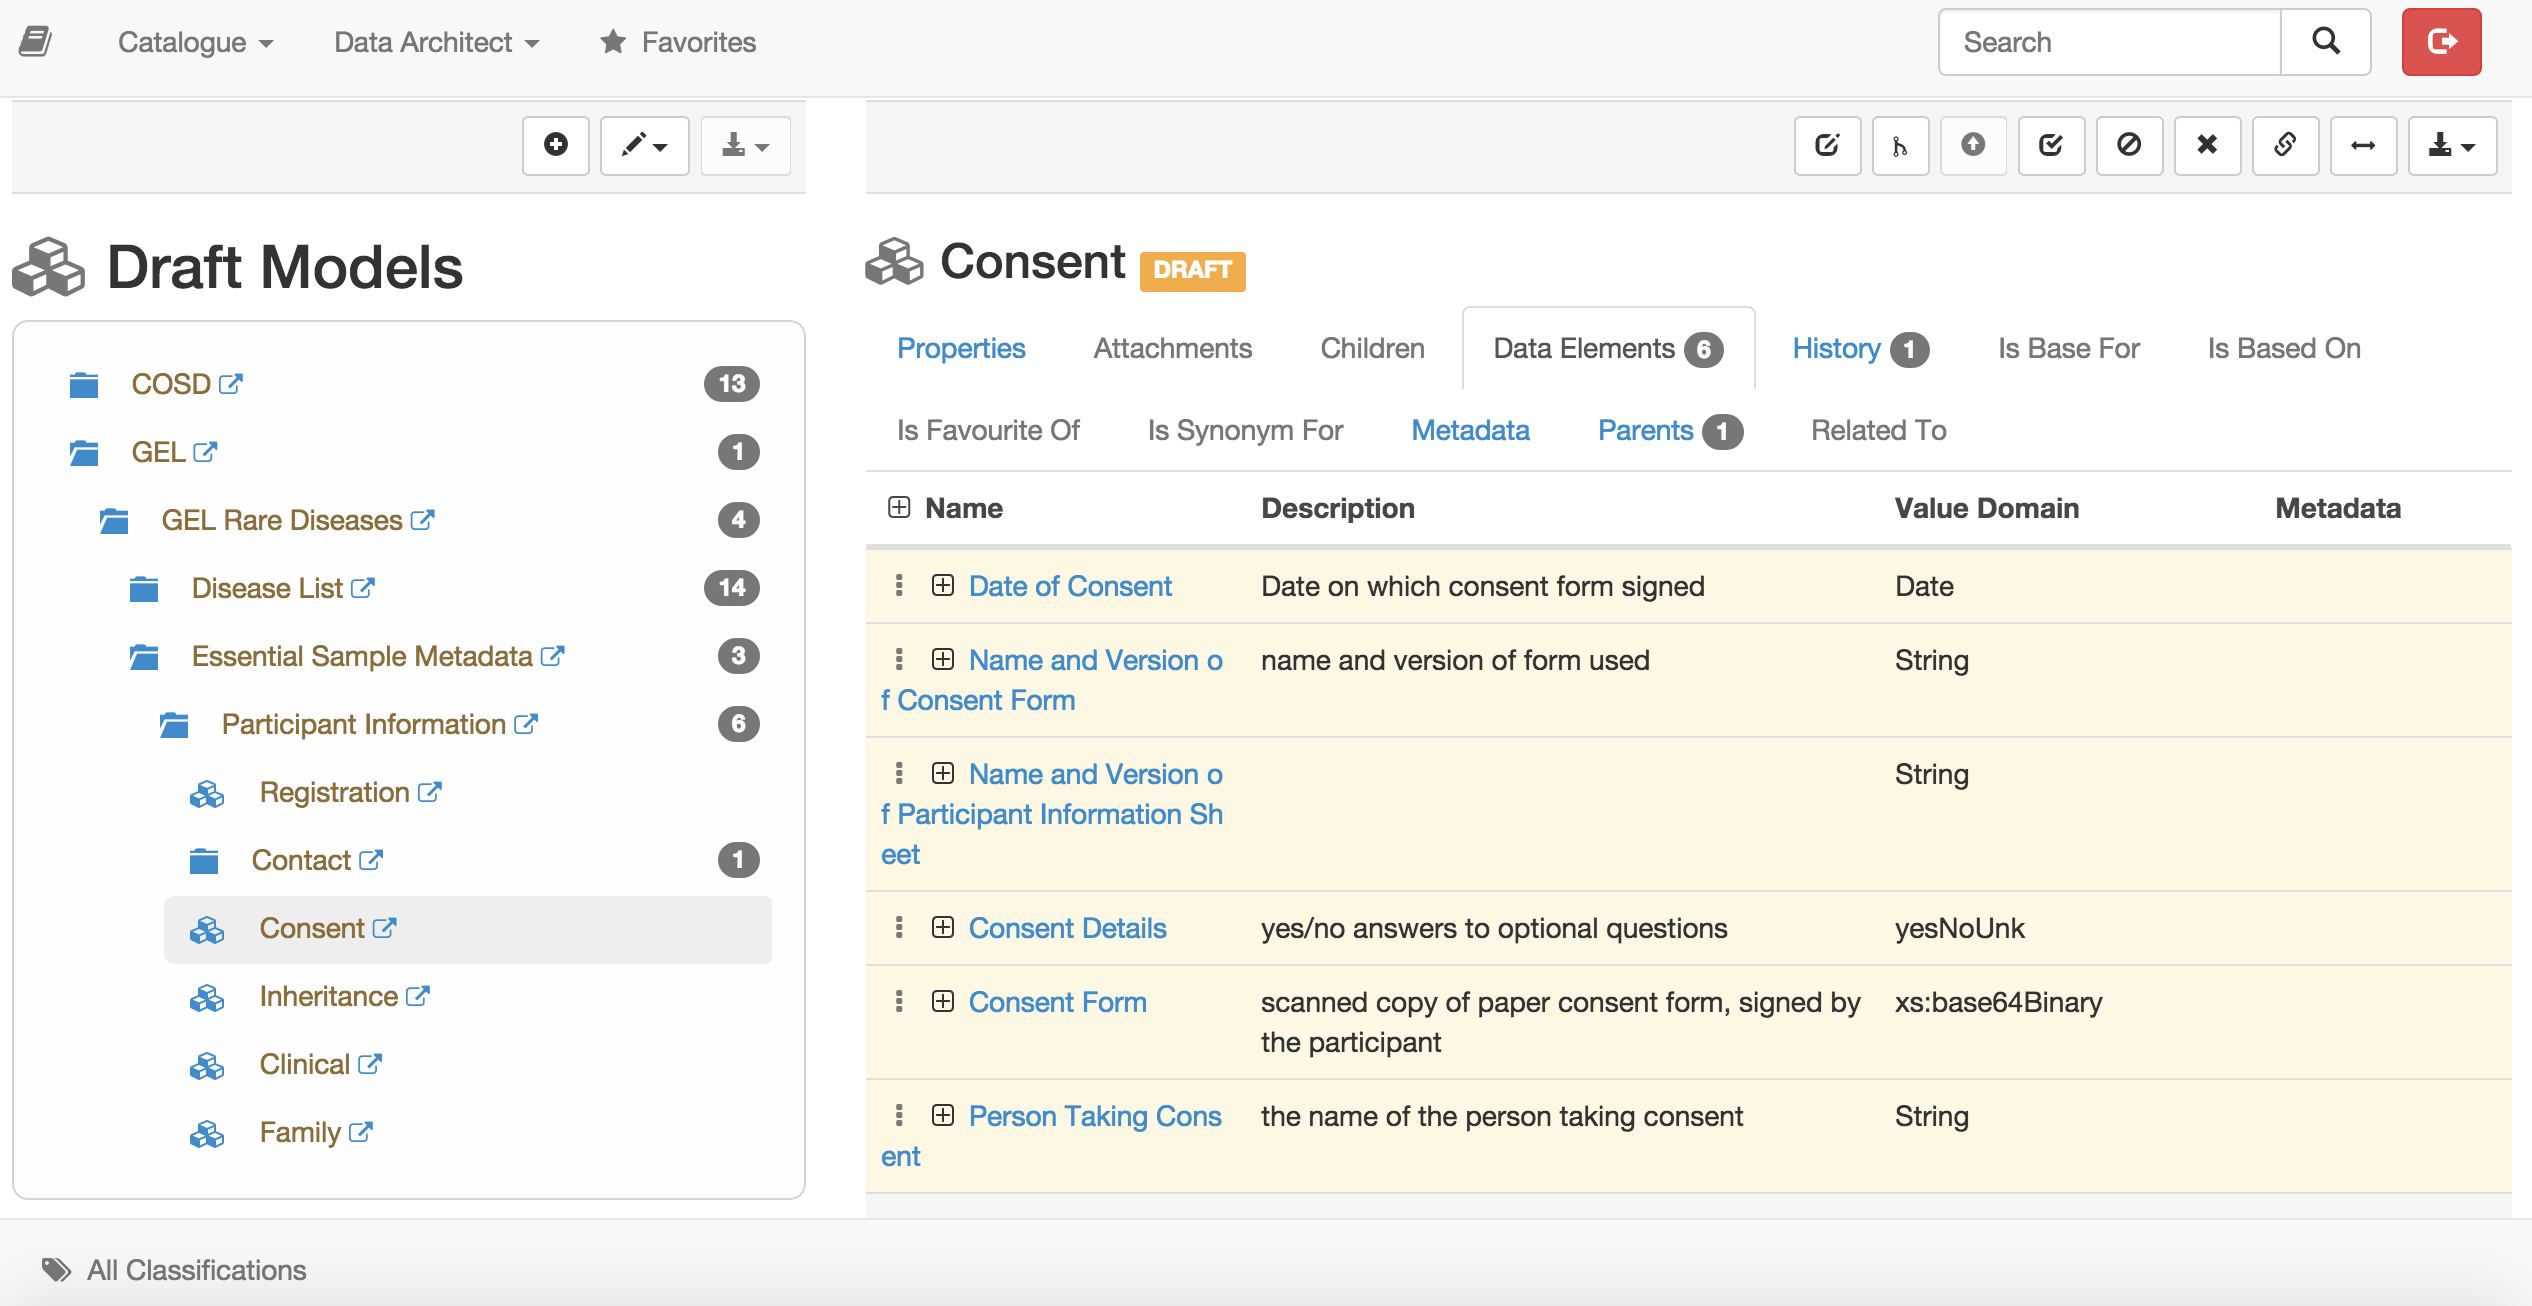
\includegraphics[width=\textwidth]{ScreenShot1}
  \caption{web interface to the model catalogue}
  \label{fig:webinterface}
\end{figure*}

\begin{figure*}[h]
  \centering
  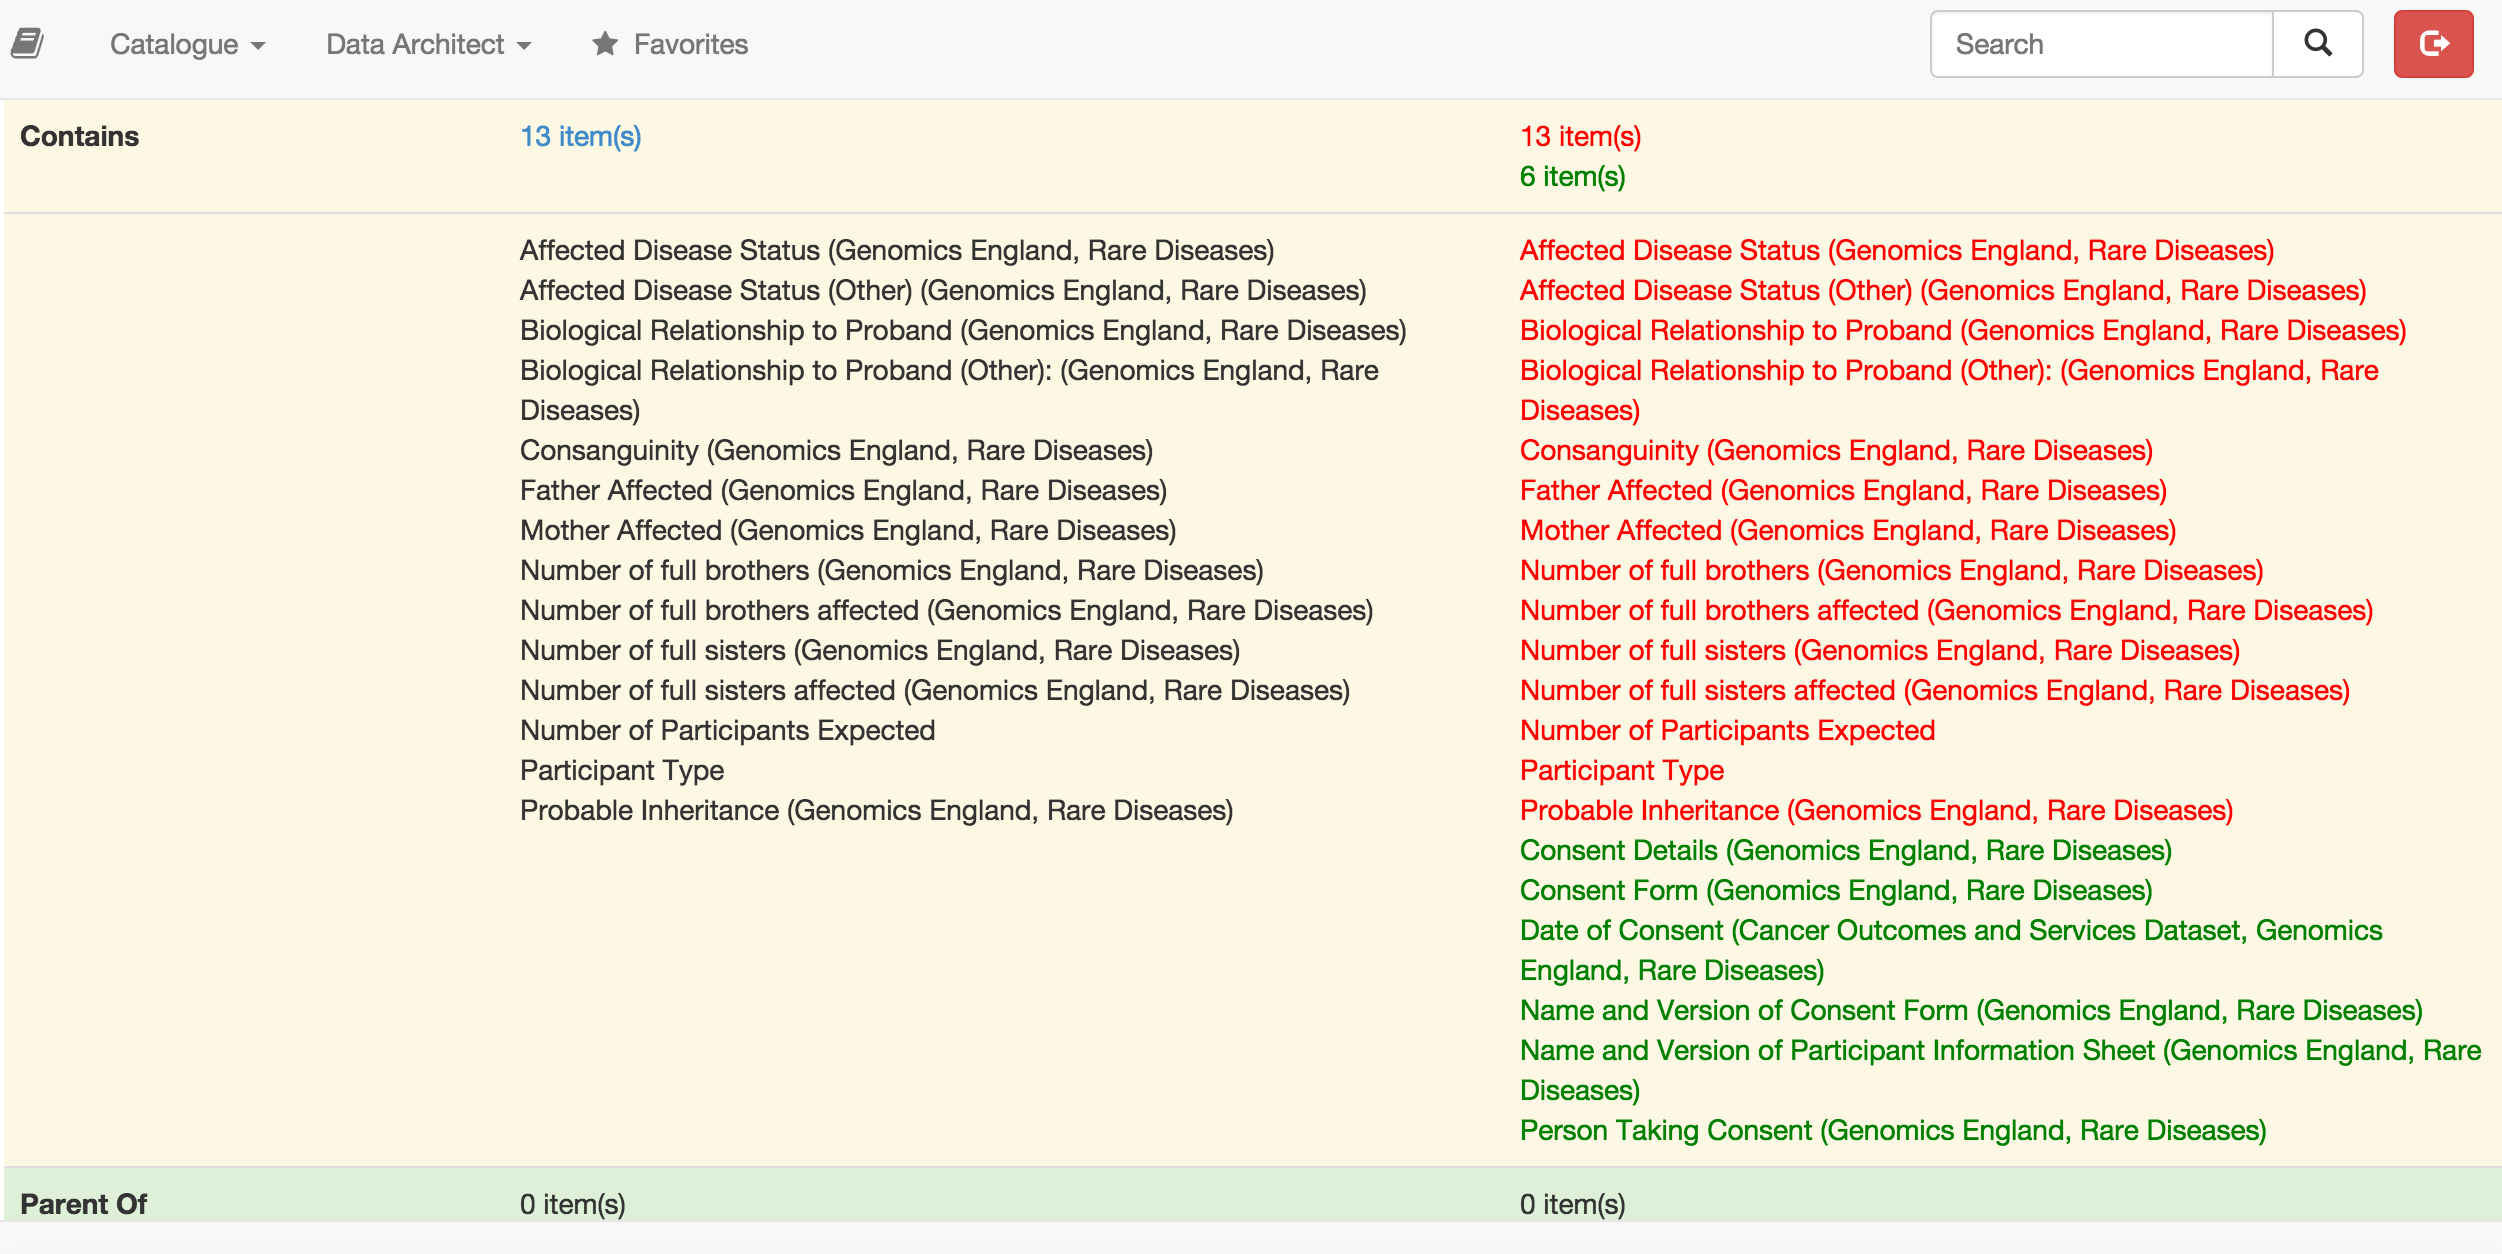
\includegraphics[width=\textwidth]{ScreenShot2}  
  \caption{automatic detection of model variation}
  \label{fig:variation}
\end{figure*}

